%%%%%%%%%%%%%%%%%%%%%%%%%%%%%%%%%%%%%%%
% Wenneker Resume/CV
% LaTeX Template
% Version 1.1 (19/6/2016)
%
% This template has been downloaded from:
% http://www.LaTeXTemplates.com
%
% Original author:
% Frits Wenneker (http://www.howtotex.com) with extensive modifications by 
% Vel (vel@LaTeXTemplates.com)
%
% License:
% CC BY-NC-SA 3.0 (http://creativecommons.org/licenses/by-nc-sa/3.0/
%
%%%%%%%%%%%%%%%%%%%%%%%%%%%%%%%%%%%%%%

%----------------------------------------------------------------------------------------
%	PACKAGES AND OTHER DOCUMENT CONFIGURATIONS
%----------------------------------------------------------------------------------------

\documentclass[a4paper,10pt]{memoir} % Font and paper size

%%%%%%%%%%%%%%%%%%%%%%%%%%%%%%%%%%%%%%%%%
% Wenneker Resume/CV
% Structure Specification File
% Version 1.1 (19/6/2016)
%
% This file has been downloaded from:
% http://www.LaTeXTemplates.com
%
% Original author:
% Frits Wenneker (http://www.howtotex.com) with extensive modifications by 
% Vel (vel@latextemplates.com)
%
% License:
% CC BY-NC-SA 3.0 (http://creativecommons.org/licenses/by-nc-sa/3.0/)
%
%%%%%%%%%%%%%%%%%%%%%%%%%%%%%%%%%%%%%%%%%

%----------------------------------------------------------------------------------------
%	PACKAGES AND OTHER DOCUMENT CONFIGURATIONS
%----------------------------------------------------------------------------------------

\usepackage{lato} % Use the Bitstream Charter font
\usepackage[utf8]{inputenc} % Required for inputting international characters
\usepackage[T1]{fontenc} % Output font encoding for international characters

\usepackage[top=2cm,left=1cm,right=1cm,bottom=2cm]{geometry} % Modify margins

\usepackage{graphicx} % Required for figures

\usepackage{flowfram} % Required for the multi-column layout

\usepackage{url} % URLs
\usepackage{hyperref}

\usepackage[usenames,dvipsnames]{xcolor} % Required for custom colours

\usepackage{tikz} % Required for the horizontal rule

\usepackage{enumitem} % Required for modifying lists
\setlist{noitemsep,nolistsep} % Remove spacing within and around lists

\setlength{\columnsep}{\baselineskip} % Set the spacing between columns

% Define the left frame (sidebar)
\newflowframe{0.2\textwidth}{\textheight}{0pt}{0pt}[left]
\newlength{\LeftMainSep}
\setlength{\LeftMainSep}{0.2\textwidth}
\addtolength{\LeftMainSep}{1\columnsep}
 
% Small static frame for the vertical line
\newstaticframe{1.5pt}{\textheight}{\LeftMainSep}{0pt}
 
% Content of the static frame with the vertical line
\begin{staticcontents}{1}
\hfill
\tikz{\draw[loosely dotted,color=RoyalBlue,line width=1pt,yshift=0](0,0) -- (0,\textheight);}
\hfill\mbox{}
\end{staticcontents}
 
% Define the right frame (main body)
\addtolength{\LeftMainSep}{1.5pt}
\addtolength{\LeftMainSep}{1\columnsep}
\newflowframe{0.7\textwidth}{\textheight}{\LeftMainSep}{0pt}[main01]

\pagestyle{empty} % Disable all page numbering

\setlength{\parindent}{0pt} % Stop paragraph indentation

%----------------------------------------------------------------------------------------
%	NEW COMMANDS
%----------------------------------------------------------------------------------------

\newcommand{\userinformation}[1]{\renewcommand{\userinformation}{#1}} % Define a new command for the CV user's information that goes into the left column

\newcommand{\cvheading}[1]{{\Huge\bfseries\color{RoyalBlue} #1} \par\vspace{.6\baselineskip}} % New command for the CV heading
\newcommand{\cvsubheading}[1]{{\Large\bfseries #1} \bigbreak} % New command for the CV subheading

\newcommand{\Sep}{\vspace{0.8em}} % New command for the spacing between headings
\newcommand{\SmallSep}{\vspace{0.5em}} % New command for the spacing within headings

\newcommand{\aboutme}[2]{ % New command for the about me section
\textbf{\color{RoyalBlue} #1}~#2\par\Sep
}
	
\newcommand{\CVSection}[1]{ % New command for the headings within sections
{\Large\textbf{#1}}\par
\SmallSep % Used for spacing
}

\newcommand{\CVItem}[3]{ % New command for the item descriptions
\textbf{\color{RoyalBlue} #1 \hfill {#2}}
\par
#3
\SmallSep % Used for spacing
}

\newcommand{\bluebullet}{\textcolor{RoyalBlue}{$\circ$}~~} % New command for the blue bullets
 % Include the file specifying document layout and packages

%----------------------------------------------------------------------------------------
%	NAME AND CONTACT INFORMATION 
%----------------------------------------------------------------------------------------

\userinformation{ % Set the content that goes into the sidebar of each page
\begin{flushright}
% Comment out this figure block if you don't want a photo
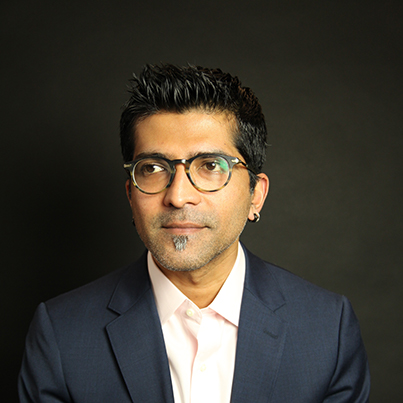
\includegraphics[width=0.6\columnwidth]{shameel_portrait_2017_small.jpg}\\[\baselineskip] % Your photo
\small % Smaller font size
Shameel Arafin \\ % Your name
shameel@arafin.net \\ % Your email address
\href{http://www.shameelarafin.com/}{shameelarafin.com} \\ % Your URL
(215) 982-0854 \\ % Your phone number
\Sep % Some whitespace
\textbf{LinkedIn} \\
\href{http://www.linkedin.com/in/shameelarafin/}{shameelarafin} \\ % Address 1
% United States \\ % Address 3
\vfill % Whitespace under this block to push it up under the photo
\end{flushright}
}

%----------------------------------------------------------------------------------------

\begin{document}

\userinformation % Print your information in the left column

\framebreak % End of the first column

%----------------------------------------------------------------------------------------
%	HEADING
%----------------------------------------------------------------------------------------

\cvheading{Shameel Arafin} % Large heading - your name

% \cvsubheading{Technology Executive} % Subheading - your occupation/specialization

%----------------------------------------------------------------------------------------
%	ABOUT ME
%----------------------------------------------------------------------------------------

\aboutme{Executive}{with extensive strategic and operational experience in technology, education, media and finance. Consensus-builder in high-pressure environments, project manager at scale. Recent domain expertise focused on machine learning/artificial intelligence; digital journalism (platform/CMS, and storytelling), and EdTech. Leader, educator, mentor, engineering gender-parity advocate. 10+ years in digital strategy, web development, product management and large-scale project development. Former investment banker.}

%----------------------------------------------------------------------------------------
%	EXPERIENCE
%----------------------------------------------------------------------------------------

\CVSection{Experience}

%------------------------------------------------
\CVItem{CUNY, New Jersey Institute of Technology}{Winter 2015 - Present}{\textit{Data Science \& Artificial Intelligence Research/Instructor}}
\begin{itemize}
	\item Tech-In-Residence Corps: Working to fulfill Mayor's goal of supporting a pipeline of local talent pursuing tech degrees at CUNY. Developing curriculum and will be teaching survey on machine learning and data science at Lehman College as Adjunct Professor starting January 2019.

	\item CUNY 2X Tech Working Group: Advising Tech Talent Pipeline (TTP) on syllabus, boot camp process, and strategy. Advising CUNY computer science departments on syllabus.

	\item Consulting with NJIT's Director of Data Science and Bioinformatics. Researching machine learning algorithms for fake news detection.
\end{itemize}

\Sep % Extra whitespace after the end of a major section

%------------------------------------------------

\CVItem{Meredith Corp. (formerly Time Inc.)}{August 2015 - February 2018}{\textit{Senior Director, Platform Engineering, News Group}}
\begin{itemize}
	\item Led engineering teams for News, Health and Education verticals, as well as branded content/native advertising efforts. Delivered multimillion-dollar engagements, working closely with editorial, advertising and marketing teams. Clients included \href{http://time.com/paid-content-from/netflix/dinnertime/}{Netflix} and \href{http://time.com/partner/siemens/innovation-starts-here/}{Siemens} (seven-figure engagement).

	\item Responsible for all technological aspects of \href{http://time.com}{time.com}, \href{http://fortune.com}{fortune.com}, \href{http://money.com}{money.com}, \href{https://www.timeforkids.com}{timeforkids.com}, \href{https://www.health.com}{health.com} and other brands, at scale - a portfolio that delivered hundreds of millions of monthly unique visitors.

	\item Successfully launched multiple award-winning projects, including  \href{http://time.com/time-person-of-the-year-2017-silence-breakers/}{TIME's Person of the Year ``The Silence Breakers"} and \href{http://time.com/finding-home/}{``Finding Home"}, winner of American Society of Magazine Editors (ASME) award, Picture of the Year (POY) award, and Edward R. Murrow award; Emmy-nominated.

	\item Drove re-architecture, re-platforming and development of \href{https://www.timeforkids}{Time For Kids}, transforming it into an EdTech learning management system (LMS). Features include multiple lexile levels, translations, audio read-aloud, and online-assessment.

	\item Launched multiple  \href{https://medium.com/@acharalambides/element-the-digital-unification-of-time-inc-979656149fd3}{re-designs} of News, Education and Health brands.

	\item Recruited and led over a dozen developers, growing a team from 2 to 14 members, whose composition approached gender parity (43\% female). Deeply involved in mentoring throughout the company, in Product, Design and Engineering departments. 
\end{itemize}
\Sep % Extra whitespace after the end of a major section


%------------------------------------------------
\CVItem{MediaStorm}{June 2011 - July 2015}{\textit{Platform Architect \& Lead Developer}}
\begin{itemize}
	\item Created architecture and back-end development for MediaStorm Platform, a cinematic, interactive storytelling tool. 
	\item First online video player to \href{http://time.com/46716/game-changer-mediastorm-launches-pay-per-story-video-player/}{implement transaction (pay to view)}, built on proprietary CMS --- featured in TIME magazine. Key users/clients include \href{https://mediastorm.com/clients/2018-icp-infinity-awards}{Wall Street Journal}, \href{https://mediastorm.com/clients/sundance-short-film-challenge}{Sundance Institute}, \href{https://mediastorm.com/clients/i-am-not-who-they-think-i-am-for-ictj}{International Center for Transitional Justice}. 
	\item Led technology sections for MediaStorm Workshops.
	\item Recruited developers and interns. Initiated 401(k) plan.
\end{itemize}
\Sep % Extra whitespace after the end of a major section

\clearpage % Start a new page
\userinformation % Print your information in the left column
\framebreak % End of the first column


%------------------------------------------------
\CVItem{SignalFive}{September 2008 - June 2011}{\textit{Co-Founder, CTO}}
\begin{itemize}
	\item Co-founded SignalFive, an interactive design, development and strategy agency for web and mobile apps. Responsibilities included all aspects of entrepreneurship, from accounting (developed proprietary in-house invoicing system) to business development (led eight interns one summer) to RFPs (pitched FreshDirect).

	\item Clients included Al Gore's \href{https://www.climaterealityproject.org/}{Alliance for Climate Protection}. Built a multimedia app driven by citizen- and documentary video journalism.

	\item As an agency, developed various iPhone apps for clients such as Grand Marnier. Architected and coded prototype of PopStay, a social app for vacation-rentals and home-swapping (before AirBnB became the gorilla in the space).
\end{itemize}
\Sep % Extra whitespace after the end of a major section

%------------------------------------------------

\CVItem{Massify}{September 2007 - September 2008}{\textit{Developer, Project Manager}}
\begin{itemize}
	\item Back-end developer at Icahn-funded startup, a social network/crowd-sourcing \href{https://www.nytimes.com/2008/03/10/business/media/10massify.html}{web application} for the film and TV industry.
	\item Reported to CTO, worked with team to build and launch the beta version of \href{https://www.massify.com}{Massify.com}, which launched in November 2007, followed by a full launch a few months later. 
\end{itemize}
\Sep % Extra whitespace after the end of a major section

%------------------------------------------------
\CVItem{Freelance Developer}{December 2002 - June 2008}{\textit{Software Engineer}}
\begin{itemize}
	\item Various projects, including full re-design, re-platforming and re-launch of Mercy Health System's websites throughout the greater Philadelphia area (14 websites launched simultaneously). 
\end{itemize}
\Sep % Extra whitespace after the end of a major section

%------------------------------------------------


\CVItem{Credit Suisse First Boston Tech Group}{July 1998 - March 2002}{\textit{Senior Research Associate}}
\begin{itemize}
	\item Equity research in Semiconductor Capital Equipment and Communications Test \& Measurement sectors.
\end{itemize}
\Sep % Extra whitespace after the end of a major section

%------------------------------------------------
\CVItem{Deutsche Bank Securities Tech Group}{June 1997 - July 1998}{\textit{Research Assistant}}
\begin{itemize}
	\item Research Assistant to Director of Research/Lead Analyst on PC Hardware \& Software. Editor of \textit{The Tech Daily}.
\end{itemize}

\Sep % Extra whitespace after the end of a major section

%----------------------------------------------------------------------------------------
%	MENTORSHIP/TEACHING
%----------------------------------------------------------------------------------------

\CVSection{Mentorship/Teaching/Advisory}

\CVItem{High School of Art \& Design}{November 2016 - Present}{\textit{Advisory Board Member}}
\begin{itemize}
	\item Syllabus ratification per New York Department of Education.
	\item Portfolio reviews, guest speaking.
\end{itemize}

\Sep % Extra whitespace after the end of a major section


\CVItem{Mountain Workshops, Western Kentucky University}{October 2017}{\textit{Digital Storytelling \& Data Visualization Coach}}
\begin{itemize}
	\item Co-led week-long workshop with half a dozen students, using code, design, photo, video, and cartography to tell interactive, local stories.
\end{itemize}

%------------------------------------------------

\Sep % Extra whitespace after the end of a major section

%----------------------------------------------------------------------------------------
%	Certifications
%----------------------------------------------------------------------------------------

\CVSection{Certifications}

%------------------------------------------------

\CVItem{Scrum Alliance}{February 2018 - Present}{\textit{Certified Scrum Product Owner}}
\Sep % Extra whitespace after the end of a major section


%----------------------------------------------------------------------------------------
%	EDUCATION
%----------------------------------------------------------------------------------------

\CVSection{Education}

%------------------------------------------------

\CVItem{Harvard University}{September 1995 - June 1997}{A.B. Literature (Honors)}

%------------------------------------------------

\CVItem{California Institute of Technology}{September 1993 - June 1995}{Electrical Engineering / Literature candidate}

%------------------------------------------------

\Sep % Extra whitespace after the end of a major section

%----------------------------------------------------------------------------------------
%	SKILLS
%----------------------------------------------------------------------------------------

% \CVSection{Technical Skills}

%------------------------------------------------
% {\begin{tabular}{p{0.2\textwidth} p{0.2\textwidth} p{0.2\textwidth}}
% 	\bluebullet Python/Django &
% 	\bluebullet Node/Express &
% 	\bluebullet PHP/CodeIgniter\\
	
% 	\bluebullet Postgresql/MySQL &  
 % 	\bluebullet AWS &  
 % 	\bluebullet WordPress VIP\\
% \end{tabular}}
% \Sep % Extra whitespace after the end of a major section

%------------------------------------------------

%----------------------------------------------------------------------------------------
%	NEW PAGE DELIMITER
%	Place this block wherever you would like the content of your CV to go onto the next page
%----------------------------------------------------------------------------------------

% \clearpage % Start a new page
% \userinformation % Print your information in the left column
% \framebreak % End of the first column

%----------------------------------------------------------------------------------------
%	AWARDS
%----------------------------------------------------------------------------------------

% \CVSection{Awards}

%------------------------------------------------

% \CVItem{2010, \textit{Postgraduate Scholarship}, Cornell University}{Awarded to the top student in their final year of a Bachelors degree.}

%------------------------------------------------

% \Sep % Extra whitespace after the end of a major section

%----------------------------------------------------------------------------------------
%	INTERESTS
%----------------------------------------------------------------------------------------

% \CVSection{Interests}

% %------------------------------------------------

% \begin{itemize}
% 	\item Digital publishing, digital journalism 
% 	\item Interactive storytelling, documentary video, digital design
% 	\item Trail running, photography
% \end{itemize}

% \Sep % Extra whitespace after the end of a major section

%----------------------------------------------------------------------------------------

\end{document}
